\iffalse
\chapter{2021}
\author{EE24BTECH11040}
\section{ph}
\fi

\item Consider a point charge $+Q$ of mass $m$ suspended by a massless, inextensible string of length $l$ in free space (permittivity $\varepsilon_0$) as shown in the figure. It is placed at a height $d$ $(d>l)$ over an infinitely large, grounded conducting plane. The gravitational potential energy is assumed to be zero at the position of the conducting plane and is positive above the plane.

\vspace{0.5 cm}

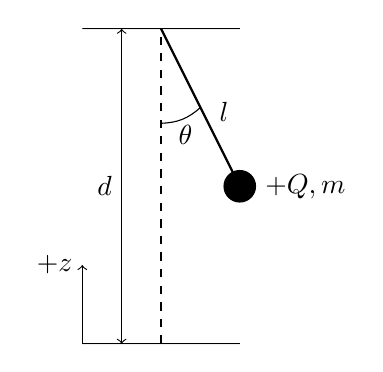
\begin{tikzpicture}
    \draw[fill=black!50] (0,0) rectangle (2,0);
    \draw[fill=black!50] (0,4) rectangle (2,4);
    \draw[dashed] (1,0) -- (1,4);
    \draw[<->] (0.5,0) -- (0.5,4) node[midway, left] {$d$};
    \draw[thick] (1,4) -- (2,2);
    \draw[fill=black] (2,2) circle (0.2);
    \node[right] at (2.2,2) {$+Q,m$};
    \draw (1,2.8) to[bend right=20] (1.5,3);
    \node[above right] at (1.1,2.4) {$\theta$};
    \node[above] at (1.8,2.7) {$l$};
    \draw[->] (0,0) -- (0,1) node[left] {$+z$};
\end{tikzpicture}

If $\theta$ represents the angular position and $p_\theta$ its corresponding canonical momentum, then the correct Hamiltonian of the system is

\begin{enumerate}
\item $\frac{p^2_\theta}{2ml^2}-\frac{Q^2}{16\pi\varepsilon_0(d-l\cos{\theta})}-mg(d-l\cos{\theta})$
\item $\frac{p^2_\theta}{2ml^2}-\frac{Q^2}{8\pi\varepsilon_0(d-l\cos{\theta})}+mg(d-l\cos{\theta})$
\item $\frac{p^2_\theta}{2ml^2}-\frac{Q^2}{8\pi\varepsilon_0(d-l\cos{\theta})}-mg(d-l\cos{\theta})$
\item $\frac{p^2_\theta}{2ml^2}-\frac{Q^2}{16\pi\varepsilon_0(d-l\cos{\theta})}+mg(d-l\cos{\theta})$
\end{enumerate}

\item Consider two concentric conducting spherical shells as shown in the figure. The inner shell has a radius $a$ and carries a charge $+Q$. The outer shell has a radius $b$ and carries a charge $-Q$. The empty space between them is half-filled by a hemispherical shell of a dielectric having permittivity $\varepsilon_1$. The remaining space between the shells is filled with air having the permittivity $\varepsilon_0$.

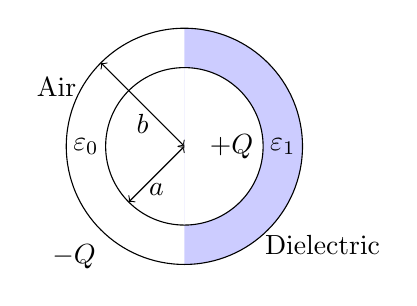
\begin{tikzpicture}
    \fill[blue!20] (0,-1.5) arc (-90:90:1.5) -- (0,-1.5) -- cycle;
    \fill[white] (0,-1) arc (-90:90:1) -- (0,-1) -- cycle;
    \draw (0,0) circle (1.5);
    \draw (0,0) circle (1);
    \node at (0.6,0) {$+Q$};
    \node at (-1.4,-1.4) {$-Q$};
    \node at (-1.25,0) {$\varepsilon_0$};
    \node at (1.25,0) {$\varepsilon_1$};
    \node[below right] at (0.9,-1) {Dielectric};
    \node[below left] at (-1.25,1) {Air};
    \draw[<->] (0,0) -- (-1.060660171779821,1.060660171779821) node[midway, below] {$b$};
    \draw[<->] (0,0) -- (-0.7071067811865475,-0.7071067811865475) node[midway, below] {$a$};
\end{tikzpicture}

The electric field at a radial distance $r$ from the center and between the shells $(a<r<b)$ is

\begin{enumerate}
\item $\frac{Q}{2\pi(\varepsilon_0+\varepsilon_1)}\frac{\hat{r}}{r^2}$ everywhere
\item $\frac{Q}{4\pi\varepsilon_0}\frac{\hat{r}}{r^2}$ on the air side and $\frac{Q}{4\pi\varepsilon_1}\frac{\hat{r}}{r^2}$ on the dielectric side
\item $\frac{Q}{2\pi\varepsilon_0}\frac{\hat{r}}{r^2}$ on the air side and $\frac{Q}{2\pi\varepsilon_1}\frac{\hat{r}}{r^2}$ on the dielectric side
\item $\frac{Q}{4\pi(\varepsilon_0+\varepsilon_1)}\frac{\hat{r}}{r^2}$ everywhere
\end{enumerate}

\vspace{1 cm}

\item For the given sets of energy levels of nuclei X and Y whose mass numbers are odd and even, respectively, choose the best suited interpretation. 

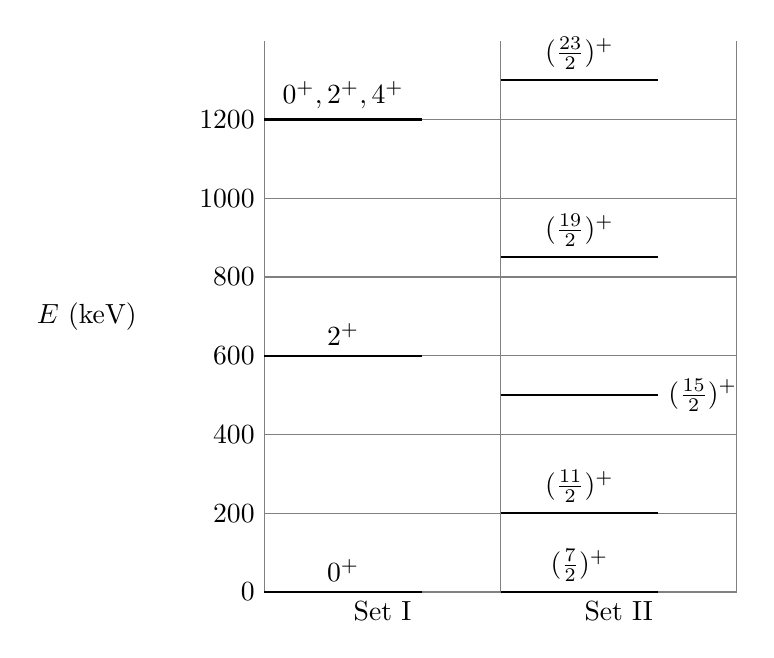
\begin{tikzpicture}
    \draw[thin, gray] (0,0) -- (0,7);
    \draw[thin, gray] (3,0) -- (3,7);
    \draw[thin, gray] (6,0) -- (6,7);
    \draw[thin, gray] (0,0) -- (6,0);
    \draw[thin, gray] (0,1) -- (6,1);
    \draw[thin, gray] (0,2) -- (6,2);
    \draw[thin, gray] (0,3) -- (6,3);
    \draw[thin, gray] (0,4) -- (6,4);
    \draw[thin, gray] (0,5) -- (6,5);
    \draw[thin, gray] (0,6) -- (6,6);
    \draw[thick] (0,0) -- (2,0) node[midway, above] {$0^+$};
    \draw[thick] (0,3) -- (2,3) node[midway, above] {$2^+$};
    \draw[thick] (0,6) -- (2,6) node[midway, above] {$0^+,2^+,4^+$};
    \draw[thick] (3,0) -- (5,0) node[midway, above] {$(\frac{7}{2})^+$};
    \draw[thick] (3,1) -- (5,1) node[midway, above] {$(\frac{11}{2})^+$};
    \draw[thick] (3,2.5) -- (5,2.5) node[right] {$(\frac{15}{2})^+$};
    \draw[thick] (3,4.25) -- (5,4.25) node[midway, above] {$(\frac{19}{2})^+$};
    \draw[thick] (3,6.5) -- (5,6.5) node[midway, above] {$(\frac{23}{2})^+$};
    \node[below] at (1.5,0) {Set I};
    \node[below] at (4.5,0) {Set II};
    \node[left] at (0,6) {1200};
    \node[left] at (0,5) {1000};
    \node[left] at (0,4) {800};
    \node[left] at (0,3) {600};
    \node[left] at (0,2) {400};
    \node[left] at (0,1) {200};
    \node[left] at (0,0) {0};
    \node[left] at (-1.5,3.5) {$E$ (keV)};
\end{tikzpicture}

\begin{enumerate}
\item Set I: Rotational band of X \\ Set II: Vibrational band of Y
\item Set I: Rotational band of Y \\ Set II: Vibrational band of X
\item Set I: Vibrational band of X \\ Set II: Rotational band of Y
\item Set I: Vibrational band of Y \\ Set II: Rotational band of X
\end{enumerate}

\item Consider a system of three distinguishable particles, each having spin $S=\frac{1}{2}$ such that $S_z=\pm\frac{1}{2}$ with corresponding magnetic moments $\mu_z=\pm\mu$.When the system is placed in an external magnetic field $H$ pointing along the z-axis, the total energy of the system is $\mu H$. Let $x$ be the state where the first spin has $S_z=\frac{1}{2}$. The probability of having the state $x$ and the mean magnetic moment (in the $+z$ direction) of the system in state $x$ are

\begin{enumerate}
\item $\frac{1}{3}$, $-\frac{1}{3}\mu$
\item $\frac{1}{3}$, $\frac{2}{3}\mu$
\item $\frac{2}{3}$, $-\frac{2}{3}\mu$
\item $\frac{2}{3}$, $\frac{1}{3}\mu$
\end{enumerate}

\item Consider a particle in a one-dimensional infinite potential well with its walls at $x=0$ and $x=L$. The system is perturbed as shown in the figure.

\begin{tikzpicture}
    \draw[thick] (0,0) -- (0,3);
    \draw[thick] (3,2) -- (3,3);
    \draw[dashed] (0,3) -- (0,4);
    \draw[dashed] (3,3) -- (3,4);
    \draw[dashed] (0,0) -- (3,0);
    \draw[dashed] (3,0) -- (3,2);
    \draw[thick, blue] (0,0) -- (3,2);
    \node[left] at (0,0.2) {$V(0) = 0$};
    \node[below] at (3,0) {$x = L$};
    \node[below] at (0,0) {$x = 0$};
    \node[right] at (3,2) {$V(L) = V_0$};
    \node[above] at (3,4) {$\infty$};
    \node[above] at (0,4) {$\infty$};
\end{tikzpicture}

The first order correction to the energy eigenvalue is

\begin{enumerate}
\item $\frac{V_0}{4}$
\item $\frac{V_0}{3}$
\item $\frac{V_0}{2}$
\item $\frac{V_0}{5}$
\end{enumerate}

\item Consider a state described by $\psi(x,t)=\psi_2(x,t)+\psi_4(x,t)$, where $\psi_2(x,t)$ and $\psi_4(x,t)$ are respectively the second and fourth normalized harmonic oscillator wave functions and $\omega$ is the angular frequency of the harmonic oscillator. The wave function $\psi(x,t=0)$ will be orthogonal to $\psi(x,t)$ at time $t$ equal to

\begin{enumerate}
\item $\frac{\pi}{2\omega}$
\item $\frac{\pi}{\omega}$
\item $\frac{\pi}{4\omega}$
\item $\frac{\pi}{6\omega}$
\end{enumerate}

\item Consider a single one-dimensional harmonic oscillator of angular frequency $\omega$, in  equilibrium at temperature $T=(k_B\beta)^{-1}$. The states of the harmonic oscillator are all non-degenerate having energy $E_n=\brak{n+\frac{1}{2}}\bar{h}\omega$ with equal probability, where $n$ is the quantum number. The Helmholtz free energy of the oscillator is

\begin{enumerate}
\item $\frac{\bar{h}\omega}{2}+\beta^{-1}\ln{\sbrak{1-e^{\beta\bar{h}\omega}}}$
\item $\frac{\bar{h}\omega}{2}+\beta^{-1}\ln{\sbrak{1-e^{-\beta\bar{h}\omega}}}$
\item $\frac{\bar{h}\omega}{2}+\beta^{-1}\ln{\sbrak{1+e^{-\beta\bar{h}\omega}}}$
\item $\beta^{-1}\ln{\sbrak{1-e^{-\beta\bar{h}\omega}}}$
\end{enumerate}

\item A system of two atoms can be in three quantum states having energies $0$, $\epsilon$ and $2\epsilon$. The system is in equilibrium at temperature $T=(k_B\beta)^{-1}$. Match the following Statistics with the Partition function.

\begin{tabular}[12pt]{ |c| c|}
    \hline
    \textbf{Statistics} & \textbf{Partition function}\\ 
    \hline
    CD: Classical (distinguishable particles) & Z1: $e^{-\beta\epsilon}+e^{-2\beta\epsilon}+e^{-3\beta\epsilon}$ \\
    \hline 
    CI: Classical (indistinguishable particles) & Z2: $1+e^{-\beta\epsilon}+2e^{-2\beta\epsilon}+e^{-3\beta\epsilon}+e^{-4\beta\epsilon}$ \\
    \hline
    FD: Fermi-Dirac & Z3: $1+2e^{-\beta\epsilon}+3e^{-2\beta\epsilon}+2e^{-3\beta\epsilon}+e^{-4\beta\epsilon}$ \\
    \hline 
    BE: Bose-Einstein & Z4: $\frac{1}{2}+e^{-\beta\epsilon}+\frac{3}{2}e^{-2\beta\epsilon}+e^{-3\beta\epsilon}+\frac{1}{2}e^{-4\beta\epsilon}$ \\
    \hline
\end{tabular}

\begin{enumerate}
\item CD:Z1, CI:Z2, FD:Z3, BE:Z4
\item CD:Z2, CI:Z3, FD:Z4, BE:Z1
\item CD:Z3, CI:Z4, FD:Z1, BE:Z2
\item CD:Z4, CI:Z1, FD:Z2, BE:Z3
\end{enumerate}

\item The free energy of a ferromagnet is given by $F=F_0+a_0(T-T_C)M^2+bM^4$, where $F_0$, $a_0$, and $b$ are positive constants, $M$ is magnetization, $T$ is the temperature, and $T_C$ is the Curie temperature. The relation between $M^2$ and $T$ is best depicted by

\begin{enumerate}
\item \begin{tikzpicture}
    \draw[->] (0,0) -- (2,0) node[right] {$T$};
    \draw[->] (0,0) -- (0,2) node[right] {$M^2$};
    \draw (1.5,0) arc (0:90:1.5cm);
    \node[below] at (1.5,0) {$T_c$};
\end{tikzpicture}
\item 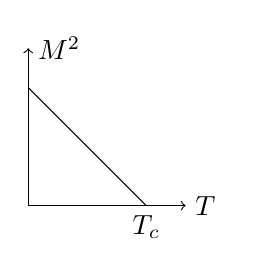
\begin{tikzpicture}
    \draw[->] (0,0) -- (2,0) node[right] {$T$};
    \draw[->] (0,0) -- (0,2) node[right] {$M^2$};
    \draw (1.5,0) -- (0,1.5);
    \node[below] at (1.5,0) {$T_c$};
\end{tikzpicture}
\item \begin{tikzpicture}
    \draw[->] (0,0) -- (2,0) node[right] {$T$};
    \draw[->] (0,0) -- (0,2) node[right] {$M^2$};
    \draw (0,0) arc (-90:0:1.5cm);
    \node[below] at (1.5,0) {$T_c$};
\end{tikzpicture}
\item \begin{tikzpicture}
    \draw[->] (0,0) -- (2,0) node[right] {$T$};
    \draw[->] (0,0) -- (0,2) node[right] {$M^2$};
    \draw (0,1.5) arc (-180:-90:1.5cm);
    \node[below] at (1.5,0) {$T_c$};
\end{tikzpicture}
\end{enumerate}

\item Consider a spherical galaxy of total mass $M$ and radius $R$, having a uniform matter distribution. In this idealized situation, the orbital speed $v$ of a star of mass $m$ $(m<<M)$ as a function of the distance $r$ from the galactic center is best described by \\ (G is the universal gravitational constant)

\begin{enumerate}
\item \begin{tikzpicture}
    \draw[->] (0,0) -- (4.2,0) node[right] {$r$};
    \draw[->] (0,0) -- (0,3) node[left] {$v$};
    \draw[dashed] (2,0) -- (2,2);
    \draw[dashed] (0,2) -- (2,2);
    \draw[thick] (0,0) -- (2,2);
    \draw[thick] (2,2) to[bend right=30] (4,0.1);
    \node[left] at (0,2) {$\sqrt{\frac{GM}{R}}$};
    \node[below] at (2,0) {$R$};
\end{tikzpicture}
\item \begin{tikzpicture}
    \draw[->] (0,0) -- (4.2,0) node[right] {$r$};
    \draw[->] (0,0) -- (0,3) node[left] {$v$};
    \draw[dashed] (2,0) -- (2,2);
    \draw[thick] (0,2) -- (2,2);
    \draw[thick] (2,2) to[bend right=30] (4,0.1);
    \node[left] at (0,2) {$\sqrt{\frac{GM}{R}}$};
    \node[below] at (2,0) {$R$};
\end{tikzpicture}
\item \begin{tikzpicture}
    \draw[->] (0,0) -- (4.2,0) node[right] {$r$};
    \draw[->] (0,0) -- (0,3) node[left] {$v$};
    \draw[dashed] (2,0) -- (2,2);
    \draw[dashed] (0,2) -- (2,2);
    \draw[thick] (0,0) -- (2,2);
    \draw[thick] (2,2) -- (4,2);
    \node[left] at (0,2) {$\sqrt{\frac{GM}{R}}$};
    \node[below] at (2,0) {$R$};
\end{tikzpicture}
\item \begin{tikzpicture}
    \draw[->] (0,0) -- (4.2,0) node[right] {$r$};
    \draw[->] (0,0) -- (0,3) node[left] {$v$};
    \draw[dashed] (2,0) -- (2,2);
    \draw[dashed] (0,2) -- (2,2);
    \draw[thick] (2,2) -- (4,2);
    \draw[thick] (0,0) to[bend right=30] (2,2);
    \node[left] at (0,2) {$\sqrt{\frac{GM}{R}}$};
    \node[below] at (2,0) {$R$};
\end{tikzpicture}
\end{enumerate}

\item Consider the potential $U(r)$ defined as $$U(r)=-U_0\frac{e^{-\alpha r}}{r}$$ where $\alpha$ and $U_0$ are real constants of appropriate dimensions. According to the first Born approximation, the elastic scattering amplitude calculated with $U(r)$ for a (wave-vector) momentum transfer $q$ and $\alpha\rightarrow0$, is proportional to \\ (Useful integral: $\int_0^\infty \sin{(qr)}e^{-\alpha r} dr=\frac{q}{\alpha^2+q^2}$)

\begin{enumerate}
\item $q^{-2}$
\item $q^{-1}$
\item $q$
\item $q^2$
\end{enumerate}

\item As shown in the figure, inverse magnetic susceptibility ($\frac{1}{\chi}$) is plotted as a function of temperature ($T$) for three different materials in paramagnetic states.

\begin{tikzpicture}
    \draw[->] (0,0) -- (6,0) node[right] {$T$};
    \draw[->] (0,0) -- (0,6) node[left] {$\frac{1}{\chi}$};
    \draw[thick, blue] (2,3) -- (5,6);
    \draw[thick, blue] (2,2) -- (5,5);
    \draw[thick, blue] (2,0) -- (5,3);
    \draw[dashed] (2,0) -- (2,3.5);
    \draw[dashed] (0,0) -- (2,2);
    \draw[dashed] (0,1) -- (2,3);
    \node[below left] at (0,0) {0};
    \node[below] at (5.1,3) {3};
    \node[below] at (5.1,5) {2};
    \node[below] at (5.1,6) {1};
\end{tikzpicture}

(Curie temperature of ferromagnetic material $=T_C$ \\ N\'eel temperature of antiferromagnetic material $=T_N$) \\ Choose the correct statement from the following

\begin{enumerate}
\item Material 1 is antiferromagnetic ($T<T_N$), 2 is paramagnetic, and 3 is ferromagnetic ($T<T_C$).
\item Material 1 is paramagnetic, 2 is antiferromagnetic ($T<T_N$), and 3 is ferromagnetic ($T<T_C$).
\item Material 1 is ferromagnetic ($T<T_C$), 2 is antiferromagnetic ($T<T_N$), and 3 is paramagnetic.
\item Material 1 is ferromagnetic ($T<T_c$), 2 is paramagnetic, and 3 is antiferromagnetic ($T<T_N$).
\end{enumerate}

\item A function $f(t)$ is defined only for $t\geq0$. The Laplace transform of $f(t)$ is $$\mathcal{L}(f;s)=\int_0^\infty e^{-st}f(t) dt$$ whereas the Fourier transform of $f(t)$ is $$\tilde{f}(\omega)=\int_0^\infty f(t)e^{-i\omega t}dt$$ The correct statement(s) is (are)

\begin{enumerate}
\item The variable $s$ is always real.
\item The variable $s$ can be complex.
\item $\mathcal{L}(f;s)=\int_0^\infty e^{-st}f(t) dt$ and $\tilde{f}(\omega)=\int_0^\infty f(t)e^{-i\omega t}dt$ can never be made connected.
\item $\mathcal{L}(f;s)=\int_0^\infty e^{-st}f(t) dt$ and $\tilde{f}(\omega)=\int_0^\infty f(t)e^{-i\omega t}dt$ can be made connected.
\end{enumerate}
